\documentclass[11pt]{article}
\usepackage{mypackages}
\begin{document}
\section{Policy Gradient Methods}

In the last section we discussed how to update the value function dynamically. Now, we will consider how to learn a \textit{parameterized policy}, $\pi (a | s, \theta)$, for computing the probability for taking action $a$ in state $s$ under policy $\pi$ without estimating any value function. The advantage of using a parameterized policy is that it is possible to solve problems that consist of continuous state and action spaces\cite{policyGrad}.

In policy gradient methods we use a
parameterized function for computing the state-action probabilities, with parameters we denote as $\theta \in \mathbb{R}^{n}$. To improve the policy we update the weights, $\theta$, by computing the gradient of a differentiable performance measure, $\rho$, with respect to the policy weights. $\theta$, 
\begin{equation}
    \theta_{t + 1} = \theta_{t} + \alpha \nabla \rho (\theta_{t})
\end{equation}
The performance measure is a function used for evaluating the performance of the parameterized policy.
The simplest performance measure is the value function for an entire run through an episode
\begin{equation}
    \rho (\theta) = v_{\pi_{\theta}}(s_{0})
\end{equation}
The parameters can be structured arbitrarily, as long as $\pi(a | s, \theta)$ is differentiable with respects to $\theta$ \cite{RLbook}.
\\ \\
The environments used in this project all consists of a continuous state space, and a discrete action space.
One challenge by using a parameterized policy combined with a discrete action space is to ensure that the policy never becomes deterministic - that is $\pi (a|s,\theta) \in (0,1)$ $\forall s, a, \theta$.
A way to solve this problem is to use a numerical preferences $h(s, a, \theta) \in \mathbb{R}$ for each state-action pair in each state. 
We can then use a function loke the softmax function to make sure the probabilities for the actions are never 0 - 1,
\begin{equation}
    \pi(a | s, \theta) = \frac{e^{h(s,a,\theta)}}{\sum_{a} e^{h(s,a,\theta)}}
\end{equation}
and,
\begin{equation}
    \sum_{a} \pi (a | s, \theta) = 1
\end{equation}

Now we have seen how we can construct a parameterized policy,
but as in section \ref{sec:td}, 
we can also create a parameterized value function. Methods that learn both a parameterized policy and a parameterized value function we mostly consider as \textit{Actor-Critic methods}.

\subsection{Actor-Critic Methods}

Actor-Critic methods are a type of policy gradient methods, that estimate both a state-value function $\hat{v}(s, \mathbf{w})$ and a parameterized policy $\pi(a | s, \theta)$. Actor-Critic methods use the value function, for update the policy, which can be seen as a critic evaluating the performance of an actor.

\begin{figure}[!h]
    \centering
    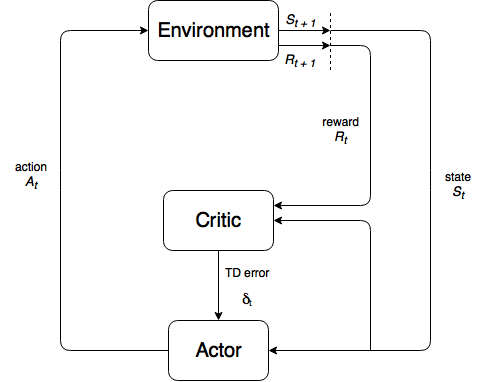
\includegraphics[scale = 0.5]{include/ActorCriticDiagram.png}
    \caption{A representation of the workflow in an Actor-Critic
    model. The environment sends a state and reward signal to both the actor and the critic. The critic compute the TD-error which is sent to the actor,
and then the actor perform a action and so forth.}
    \label{fig:actor-critic}
\end{figure}

The general idea in Actor-Critic methods is that the actor selects an action following policy $\pi$, which means it can be sampled from the distribution of the policy,
\begin{equation}
    A_{t} \sim \pi(\cdot | S_{t}, \theta_{t})
\end{equation}

Performing action $A$ results in a transition from state $S$ to state $S'$ and a corresponding reward $R$. The critic can use this information to evaluate the actor, which it does by computing the td-error,
\begin{equation}
    \delta \leftarrow R + \gamma \hat{v} (S', \mathbf{w}) - \hat{v}(S, \mathbf{w})
\end{equation}
Given the td-error it is possible to update the parameters of the policy as,
\begin{equation}
\begin{split}
    \theta &\leftarrow \theta + \delta \nabla_{\theta} \text{ log } \pi(A | S, \theta)
\end{split}
\end{equation}
and the state-value function,
\begin{equation}
\begin{split}
    \mathbf{w} &\leftarrow \mathbf{w} + \delta \nabla_{\mathbf{w}} \hat{v}(S, \mathbf{w})
\end{split}
\end{equation}
since the td-error describes the difference in our current prediction of 
$V(S_{t}, \theta)$ and the bootstrapped estimate $R_{t+1} + \gamma 
V(S_{t+1}, \theta)$, and $\mathbf{w}$ is the weight vector used for the parameterized state-value function.
An advantage when using Actor-Critic methods is that the critic is an external supervisor that returns an error measure, which is used to adjust the policy. This split reduces the variance of the function approximation, because the parameterized policy being evaluated and adjusted by the critic\cite{actCrit}, and not the actor. 


\subsection{Actor-Critic with Eligibility Traces}

In this project we using the \textit{Actor-Critic with eligibility traces}, which follow the workflow from figure \ref{fig:actor-critic}, and using eligibility traces for performing online updates of the weight vectors $\theta$ and $\mathbf{w}$. The general updating scheme for the eligibility vector $\mathbf{e}^{\mathbf{w}}$ is,
\begin{equation}
    \mathbf{e}^{\mathbf{w}} \leftarrow \lambda^{\mathbf{w}} \mathbf{e}^{\mathbf{w}} + \nabla_{\mathbf{w}} \hat{v}(S, \mathbf{w})
\end{equation}
and $\mathbf{e}^{\theta}$ as,
\begin{equation}
    \mathbf{e}^{\theta} \leftarrow \lambda^{\theta} \mathbf{e}^{\theta} + \nabla_{\theta} \text{log} \pi (A | S, \theta)
\end{equation}
where $\lambda$ discussed in section \ref{sec:td} is the discount rate, there represent how much the existing eligibility trace influence the update.
\\
The reason for using eligibility traces in Acotr-Critic methods is that it as elegant way for using the knowledge of how the gradients have changed in the last minor time period.

We have implemented Actor-Critic using Eligibility traces, and we follow this algorithm,\cite{RLbook}
\begin{algorithm}[!h]
\SetAlgoLined
    Input: a differentiable policy parameterization $\pi(a | s, \theta), \forall a \in \mathcal{A}, s \in \mathcal{S}, \theta \in \mathbb{R}^{n}$\\
    Input: a differentiable state-value parameterization  $\hat{v}(s, \mathbf{w}), \forall s \in \mathcal{S}, \mathbf{w} \in \mathbb{R}^{m}$\\
    Parameters: step sizes $\alpha > 0, \beta > 0$ \\
    Initialize policy weights $\theta$ and state-value weights $\mathbf{w}$ 

 \While{True}{
  Initialize $S$ (first state of episode) \\
$\mathbf{e}^{\theta} \leftarrow 0$ (n-component eligibility trace vector) \\
$\mathbf{e}^{\mathbf{w}} \leftarrow 0$ (m-component eligibility trace vector) \\
$I \leftarrow 1$ \\
\While{$S$ is not terminal}{    
$A \sim \pi(\cdot | S, \theta)$ \\
Take action $A$, observe $S'$, $R$ \\
$\delta \leftarrow R + \gamma \hat{v} (S', \mathbf{w}) - \hat{v}(S, \mathbf{w})$ \\
$\mathbf{e}^{\mathbf{w}} \leftarrow \lambda^{\mathbf{w}} \mathbf{e}^{\mathbf{w}} + I \nabla_{\mathbf{w}} \hat{v} (S, \mathbf{w})$ \\
$\mathbf{e}^{\theta} \leftarrow \lambda^{\theta} \mathbf{e}^{\theta} + I  \nabla_{\theta} log \pi (A | S, \theta)$ :\\
$\mathbf{w} \leftarrow \mathbf{w} + \beta \delta \mathbf{e}^{\mathbf{w}}$ \\
$\theta \leftarrow \theta + \alpha \delta \mathbf{e}^{\theta}$ \\
$I \leftarrow \gamma I$ \\
$S \leftarrow S'$
    }
 }
 \caption{Actor-Critic with Eligibility Traces}
\end{algorithm}

HJÆLP MED AT LAV EN GOD AFSLUTNING PÅ DETTE EMNE MAX!!!!









%\printbibliography
%\bibliography{citations}
%\bibliographystyle{plain}
\end{document}